%=============================================================================
% IMPLEMENTATION
% What did you do to implement this idea, and what technical achievements did you make?

% ## Guidance

% You can't talk about everything. Cover the high level first, then cover important, relevant or impressive details.
%=============================================================================

\documentclass[../main.tex]{subfiles}
\graphicspath{{\subfix{../images/}}}

\begin{document}

This chapter takes all pieces from the previous chapters and places them on the board to finally bring the system to life. Majority of the project involves implementation and writing elegant, functional code; some snippets are included. The main development environment was using \citetitle{VisualStudioCode2022} on Windows 10 with essential clients, such as \textit{Git} and \textit{Node.js}, installed.

\section{Version Control}

Using version control was an important criteria for this dissertation. Despite being required, development would not have gone forward without it since it enables history, rollback, branching, and more, allowing development to be lot more flexible and less scary with many possibilities.

\subsection[Git]{Git \& GitHub}

There are different version control architectures (such as local, centralized), but Git is the most popular version control system system and uses a distributed repository architecture providing advantages over other systems like resolving conflicts, easier branching and better performance.

\begin{figure}
    \centering
    \noindent\begin{subfigure}{.48\textwidth}
    \centering
    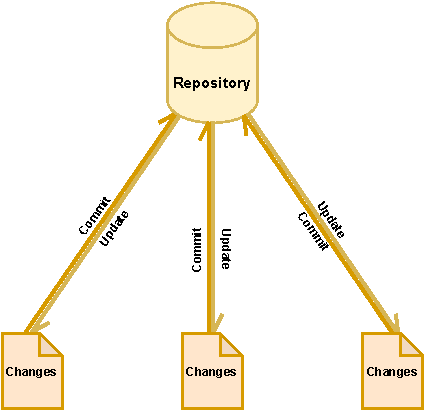
\includegraphics[width=\textwidth]{diagrams/CVCS.pdf}
    \caption{Centralised}%\label{subfig:CVCS}
    \end{subfigure}\hfill
    \begin{subfigure}{.48\textwidth}
    \centering
    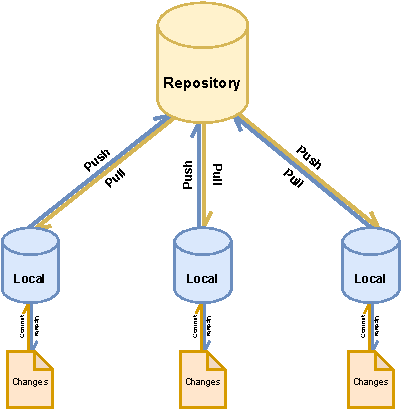
\includegraphics[width=0.95\textwidth]{diagrams/VCS.pdf}
    \caption{Distributed}%\label{subfig:DVCS}
    \end{subfigure}
    \caption{Differences between types of version control}%\label{fig:VCS}
\end{figure}

The remote repository is hosted on GitHub, which is equally popular as Git and owned by Microsoft. The service provides hosting the remote repository and displaying it as public to allow other developers to view, fork and star it; in a way it is a social network for Git repositories. The project was not public until Block 4, however. Additional features that GitHub offers for repositories on the platform include issue tracking, continuous integration and wikis \cite{GitHubPoursEnergies}. The project has taken every advantage of all features, and has also developed extensions to make the process extremely streamline (more in side projects (\ref{sec:Future Work}) and automation (\ref{subsec:Automation})).

\subsection{Issue Branching}

As issue tracking systems are industry standard, this project made sure to work with this strategy in the best possible way. It is mentioned earlier that version control (section \ref{sec:Version Control}) and Git (section \ref{subsec:Git}) enable branching that allow development to be experimental, and so all issues were worked on separate branches (named after issues, like \code{issue/19-write\_tests\_for\_api} or \code{feature/21-enable\_reverse\_logging}) so that the issue solutions can be experimental or dismissed, and the state of the repository can also be traced back easily. It avoided conflicts, and made review easier as each branch would then create a pull (or merge) request to the development trunk \code{develop}. This is heavily inspired by Atlassian products - Jira and Bitbucket - that integrate to provide issues and branching mechanism. Exposure to this system was received during an internship at \href{https://www.newverveconsulting.com/}{New Verve Consulting} in summer 2021. Pipelines were setup to enable the integration and automation (more discussed in \ref{subsec:Automation}). At the time of writing, the repository has over 60 branches (including \code{develop} and \code{master}), with 58 issues and 68 PRs closed.

\begin{figure}
    \centering
    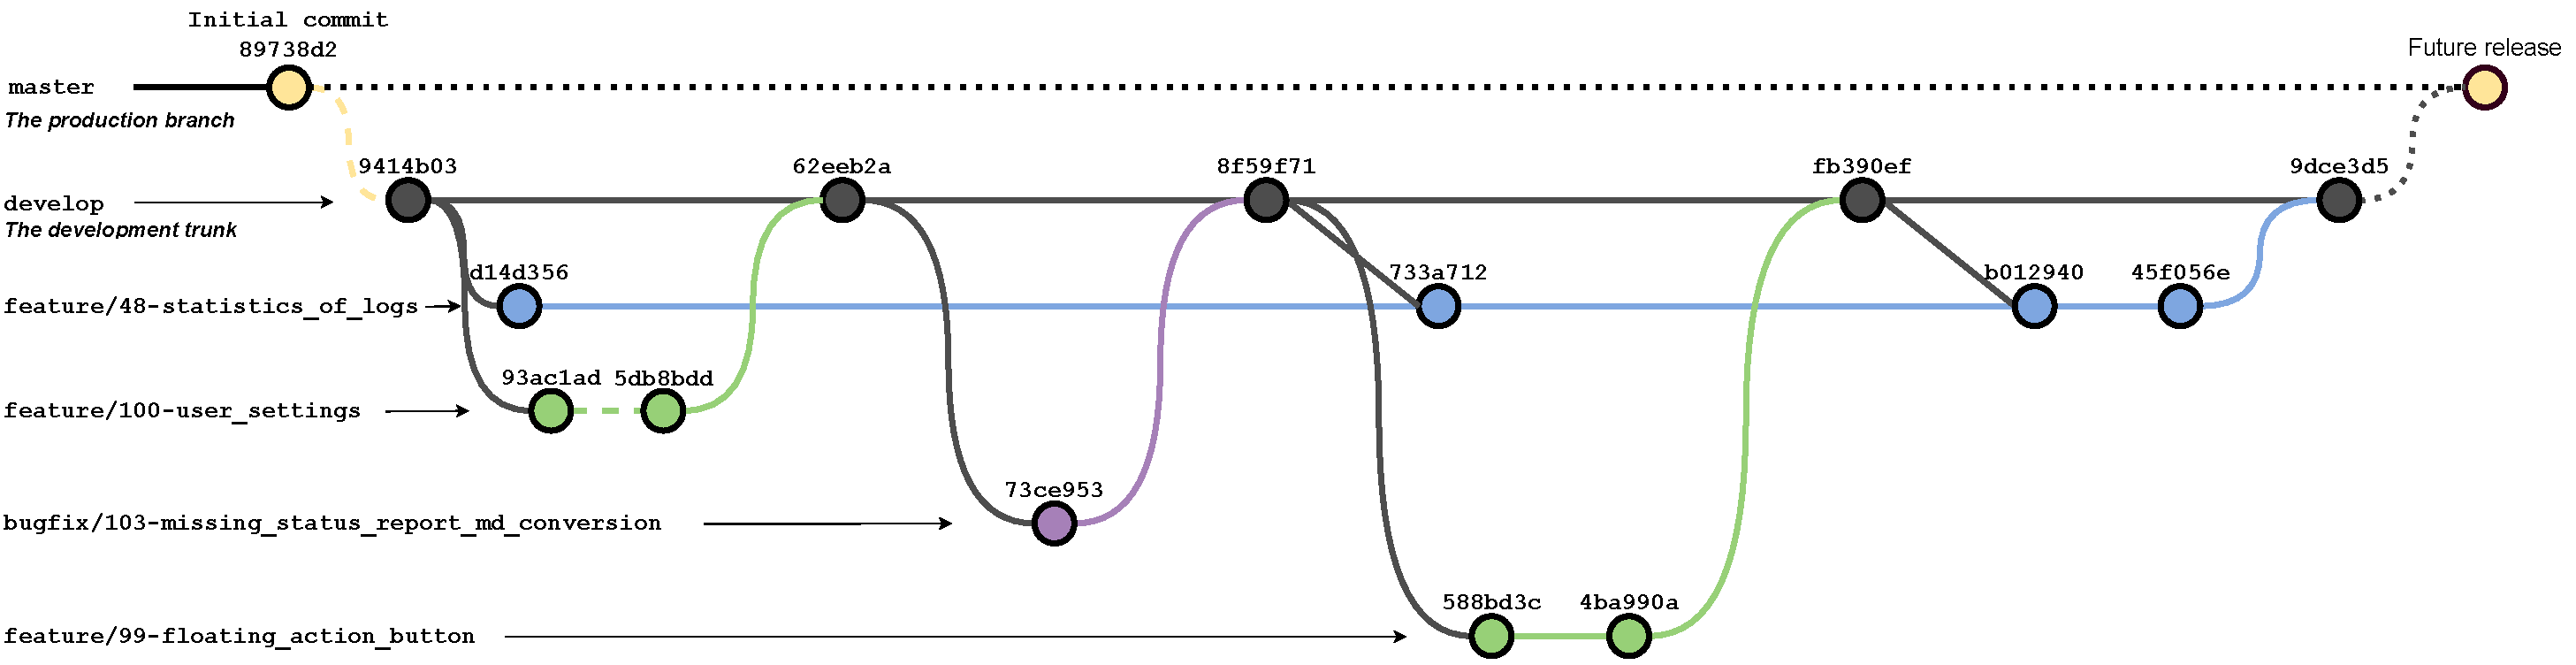
\includegraphics[width=\textwidth]{diagrams/branch_graph.pdf}
    \caption{Branch network between 23/01/22 and 30/01/22}%\label{fig:branch_graph}
\end{figure}

\begin{figure}
    \centering
    \noindent\begin{subfigure}{.49\textwidth}
    \centering
    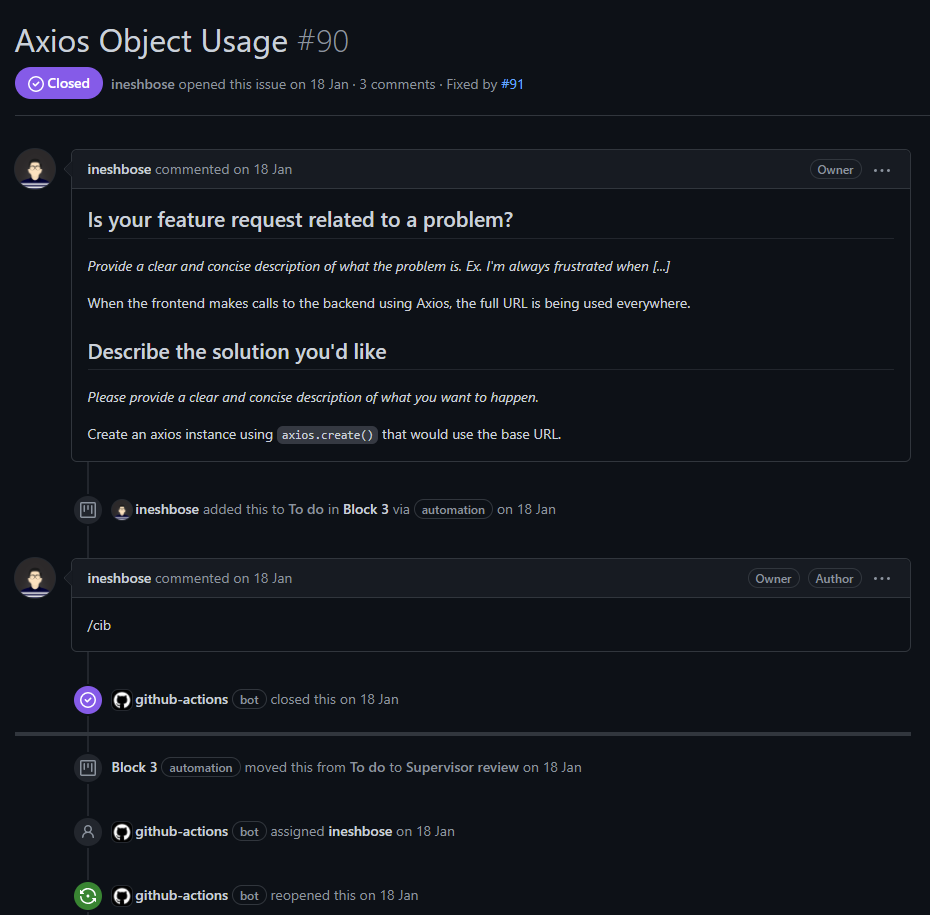
\includegraphics[width=\textwidth,trim={0 3cm 0 0},clip]{screenshots/issue_example.png}
    \caption{Issue}
    \end{subfigure}\hfill
    \begin{subfigure}{.49\textwidth}
    \centering
    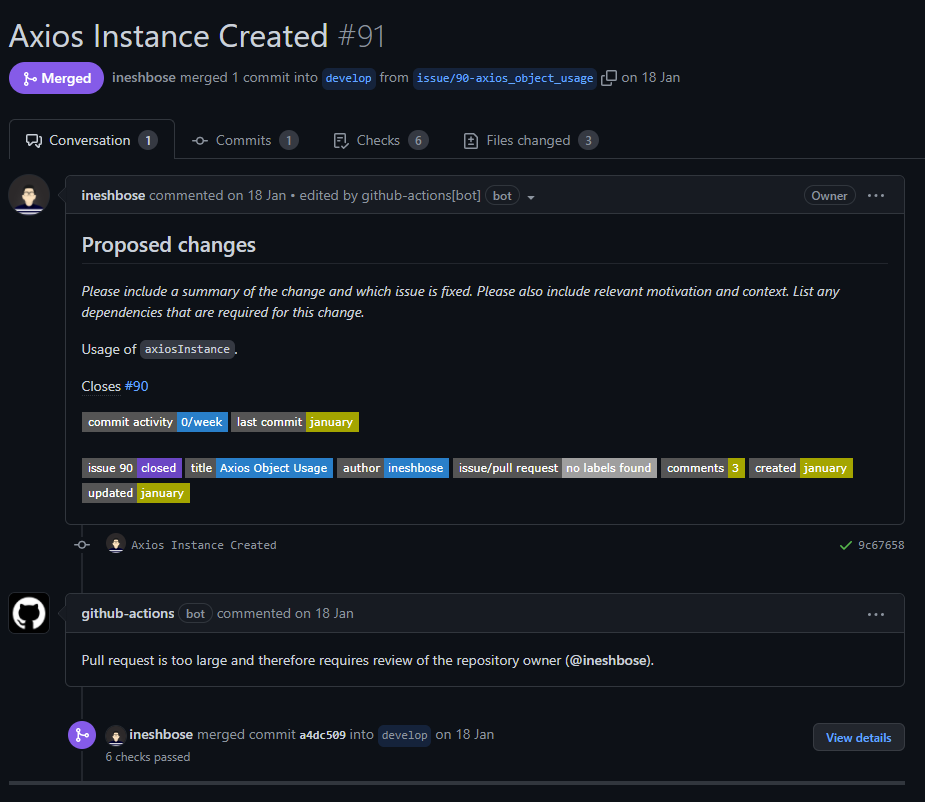
\includegraphics[width=\textwidth]{screenshots/pr_example.png}
    \caption{Pull Request}
    \end{subfigure}
    \caption{Examples of branch management using issues}%\label{fig:repo_issues_and_pr}
\end{figure}

\subsection{Hooks}

Version control systems usually provide signals (hooks) when specific commands are run. With Git \cite{gitGitHooks}, a \code{pre-commit} hook has been setup that runs the code linters (mentioned in \ref{subsubsec:Code formatting} \& \ref{subsubsec:Code styling}) before the changes can be pushed onto the remote repository (see \citecode{Issue52}). The scripts that would run on them could be setup using packages like \citecode{PrecommitPrecommit2022} and \citecode{typicodeHusky2022} - the latter being the most popular. However, husky has drawbacks such as creating additional configuration files and running an install script which may create inconsistencies for developer environments; these were not required in version 4 of the package (currently on v7 at time of writing), but the project strongly prefers packages at their latest versions, an alternate \citecode{youYorkie2022} was found (based on version 4 of husky, developed by the creator of Vue framework) that allows configuration to be in the \code{package.json} and not require installation of the script, but the package itself.

\begin{lstlisting}[language=json,caption={\citecode{PackageJson}}]
  "gitHooks": {
    "pre-commit": "npx lint-staged"
  }
\end{lstlisting}

\section{Environment setup}

As the foundation of the application, the development environment had to be configured keeping the requirements and future steps in mind. The major decision was with the languages that the stack will use that would require their own compilers and interpreters.

\subsection{Python}

A very popular programming language that many would have heard of by now. It is dynamically-typed and focuses on code readability. Learning Python is said to be easier than other languages.

\subsubsection[Pip]{Dependency Management}

\citecode{Python2022} includes the \citecode{PipPythonPackage2022} package management system that sources packages from the Python Package Index (\citetitle{PyPIPythonPackage}). This package manager, however, requires configuration that would normally be done manually using \code{pip}, like maintaing a virtual environment, updating the list of dependencies, and resolving peer-dependency version conflicts.

\begin{lstlisting}[language=bash, caption={example of \code{pip} usage}]
  $ pip install -r requirements.txt
  $ pip install requests
  $ pip freeze > requirements.txt
\end{lstlisting}

These issues have been addressed and resolved by \citetitle{PoetryDependencyManagement2022} (see \citecode{PullRequest69}) that maintains the dependencies in \code{pyproject.toml} and provide ways to make the project compatible like switching Python version easily and listing dependencies in a global way. Another similar solution is \citetitle{PipenvPythonDevelopment2022} that has some different pros and cons, but the development of Poetry is promising with the support of plugins in release version 1.12 \cite{PoetryPlugin}.

\subsubsection{Code formatting}

Python offers many different ways to write the same code, and personally, list comprehensions and inline conditions (one-liners) seem impressive, but they could make the one line of code very long and difficult to understand. To ensure that code remains consistent and readable, \citetitle{Black2022} is a formatting tool that works in compliance with PEP8 \cite{vanrossumPEPStyleGuide2001} and also produces small diffs to make code reviews faster - useful for the development strategy (discussed in \ref{subsec:Issue Branching}).

\subsection{TypeScript}

A syntactical superset of JavaScript that enables static typing, but then transpile to JavaScript to run on supported platforms. Having type definitions makes the code reliable and predictable. It auto-generates documentation for type-annotated variables and can simply be used like JavaScript with Node.js, by installing the package as a dependency.

\begin{lstlisting}[language=typescript, caption={recursive \& conditional type definition in \citecode{SrcAppTypes}}]
export type CreateData<
  T extends GenericModel | ModelID = GenericModel,
  R extends keyof T | string = 'name'
> = Partial<Omit<T, 'id' | R>> & {
  [P in R]: R extends keyof T
    ? NonNullable<T[R]> extends GenericModel | ModelID
      ? CreateData<NonNullable<T[R]>> | ModelID
      : T[R]
    : any;
};
\end{lstlisting}

\subsubsection[Yarn]{Dependency Management}

The default package manager for \citecode{NodeJs2022} is \citecode{NpmJavaScriptPackage2022} and it lists and updates dependencies in \code{package.json} automatically. In 2016, Facebook developed an alternative dubbed "Yet Another Resource Negotiator" popularly known as \citetitle{YarnpkgYarn2022} which provides better speed and stability than \citecode{Npm}. Because of this, the package manager started to be preferred by many in the community. A few years later, the development for Yarn switched to a different team therefore releasing a rewrite called \citetitle{YarnpkgBerry2022}, keeping version 1 as "Classic". Yarn Berry changed the traditional approach of resolving dependencies through a feature called "Plug'n'Play" \cite{IntroducingYarn,queirozGettingRidNode2019}. At the time of writing, the latest version of Yarn is 3.2.0. Since the approach for modern Yarn is unconventional, the project stuck to classic (see \citecode{Issue44} and \citecode{PullRequest83}). Additionally, Yarn also has a "workspaces" feature that allows the repository to use the monorepo strategy \cite{kocikYarnWorkspacesMonorepo2020,hammantTrunkBasedDevelopment,brousseIssueMonorepoPolyrepo2019,potvinWhyGoogleStores2016} and divide the codebase into modules \& packages (see \citecode{Issue71}).

\subsubsection{Code styling}

The majority of the codebase is expected to be \citecode{TypeScript2022} (which also enforces style rules onto JavaScript for type definitions) that would include React syntax (file extension \code{.[jt]sx}). All TypeScript code would be analysed using \citecode{ESLint2022} that supports ECMAScript standards to standardise and encourage compatibility \cite{stefanov2010javascript,wirfs-brockJavaScriptFirst202020}. It is the most commonly used JavaScript linter, being downloaded over 14,000,000 times per week. As mentioned, since the code is not vanilla JavaScript, additional configurations had to be added to ESLint.\footnote{File extensions written are in Regular Expression (RegEx)}

\begin{itemize}
    \item \citecode{PrettierPrettier2022} is an opinionated formatter (similar to \textit{Black} for Python - discussed in \ref{subsubsec:Code formatting}) and extends the formatting rules in ESLint with its style opinions;
    \item React is unopinionated, however a plugin for ESLint allows parsing of the HTML-like syntax and provide recommended React specific linting rules;
    \item TypeScript plugin enables ESLint to analyse \code{.tsx?} files;
    \item Airbnb defines a JavaScript Style Guide \cite{AirbnbJavascriptJavaScript} which is preferred by the community and can be setup easily along with ESLint (through \code{eslint --init}).
\end{itemize}

\subsection{Stack Specific}

\subsubsection{ngrok}

Since the application needs to be tested on mobile devices while running locally, the API calls are normally made to \code{localhost} which would not work on different devices. Therefore, the project uses a very unique, automated setup with \citetitle{shreveNgrokIntrospectedTunnels2022}\footnote{Does not use Capitalisation.} making testing incredibly easy.

\begin{lstlisting}[language=javascript, caption={Automatic ngrok connection in \citecode{SrcSetenvJs}}]
const start = (file = `${__dirname}/.env`) => {
  const env = dotenv.parse(fs.readFileSync(file, 'utf-8'));
  const port = getPort(env.API_BASE);
  if (env.DEBUG.toLowerCase() === 'true' && port) {
    ngrok.connect(port).then((value) => {
      env.API_BASE = `${value}${env.API_BASE.split(`${port}`)[1]}`;
      writeToFile(env);
    });
  } else {
    writeToFile(env);
  }
};
\end{lstlisting}

\section{Technologies}

\subsection{Django server}

The backend server of Portion Mate was developed using the \citetitle{Django2022} framework, written in Python, which follows the MVC architecture pattern \cite{FAQGeneralDjango, djangoMVC} described in \ref{subsec:Model View Controller}. The principle of this framework is \textbf{don't repeat yourself}. The framework advertises with "Batteries included" which means that it comes out of the box with libraries and utilities that could potentially be required for the development of the server, like authentication system and database connection. This could also be a downside for Django, since it makes the package bigger with modules that may be required; in that case, \citetitle{Flask2022} is an alternative. For this project, however, Django was a suitable choice. The framework arguably also follows the plug-in architecture (discussed in \ref{subsec:Plug-ins}) as it treats applications as module plugins that can be simply installed or removed through the configuration in the \code{settings.py}. Because of this, applications for Django can be distributed easily (through PyPI discussed in \ref{subsubsec:Pip}), and the project takes advantage of a few.

\subsubsection{REST Framework}

As discussed in \ref{subsec:Representational State Transfer}, the project would use a different technology for the frontend application, therefore to build a Web API, \citetitle{DjangoRESTFramework2022} was adopted. It extends Django and provides with utilities like serializers, authentication policies and a browsable API that would help visualisation JSON data. In addition to the REST architecture, Portion Mate attempted to implement a GraphQL API for more functionality (see \citecode{Issue73}).

\subsubsection{OAuth}

\textbf{O}pen \textbf{Auth}orization is an access delegation mechanism used by many major companies for their applications. Users would need to access their information such as logs, these would be provided by this method. Since the project uses API calls between the Django server and the React application, the access occurs through token (but not to be confused with JWT mechanism), which would be given on login and have an expiry.

\begin{lstlisting}[language=json, caption={Example of a web access token}]
{
    "access_token": "<your_access_token>",
    "token_type": "Bearer",
    "expires_in": 36000,
    "refresh_token": "<your_refresh_token>",
    "scope": "read write groups"
}
\end{lstlisting}

In HTTP requests, the token is added in the header as \code{Authorization}, therefore authorising requests to the user, and on expiry, these tokens can be attempted to be refreshed.

\subsubsection{PostgreSQL}

Django uses Stuctured Query Language (SQL) for database, and one would not have to write any SQL by themselves, but use functions provided by Django. The default engine for the framework is SQLite that would normally keep data in a local file (\code{db.sqlite3}), however it may introduce security vulnerabilities and problems in deployment since processes would have different versions of the file. PostgreSQL is an advanced and extensible alternative that runs on a port instead.

\subsection{React Native app}

The principle of this framework is \textbf{Learn once, write anywhere} - that translates to \textit{don't repeat yourself} (section \ref{subsec:Django server}) in writing code, programs and applications in different languages / technologies to support native applications. Instead, React Native aims to use one codebase - written in JavaScript/TypeScript, following React syntax - to support multiple platforms.

\subsubsection{Expo}

While React Native allows development of applications using React, there would be places where native development could be essential (like creating a \code{build.gradle} to publish on Android). However, \citetitle{Expo2022} removes the need for all of that and would automatically build and bundle (along with Metro) applications for cross-platform development.

\subsubsection{Axios}

Since the frontend application needs to make API requests to the server, axios\footnote{Does not require Capitalisation, based on documentation.} client was used since it automates many elements that \code{fetch} (default HTTP client) fails to do (like transforming JSON data). It supports usage of Promises in JavaScript (making usage of \code{async} and \code{await} in functions) and more versions of browsers than \code{fetch} for compatibility.

The application uses and provides a consistent, uniform and easy integrated usage of axios by using a created instance that would keep user's \code{Authorization} header (along with an attached interceptor for refreshing / revoking token) and methods that reduce code duplication.

\begin{lstlisting}[language=typescript, caption={Creation and usage of axios instance in \citecode{SrcAppApi}}]
export const axiosInstance = axios.create({
  baseURL: API_BASE,
});

// ...

export async function updateData<T extends GenericModel = GenericModel>(
  path: string,
  method: Extract<Methods, 'PATCH' | 'DELETE'>,
  data: UpdateData<T>
) {
  const { id } = data;
  const url = `${path}${id}/`;
  const response = await axiosInstance.request<T>({
    method,
    url,
    data,
  });
  return response.data;
}
\end{lstlisting}

\subsubsection{UI Kitten}

The user interface becomes the most important aspect of the application. To ensure development was easy and not requiring a lot of time and effort on just the interface, a UI component library by Akveo was chosen, and the components in this library adopted the \citetitle{EvaDesignSystem2022}, so a theme was followed throughout the application and keeping it consistent (code in \ref{lst:B.1}). As seen from figure \ref{fig:5.4}, it also made the final product similar to the wireframes (\ref{fig:4.3}).

\begin{figure}
    \centering
    \noindent\begin{subfigure}{.3\textwidth}
    \centering
    \frame{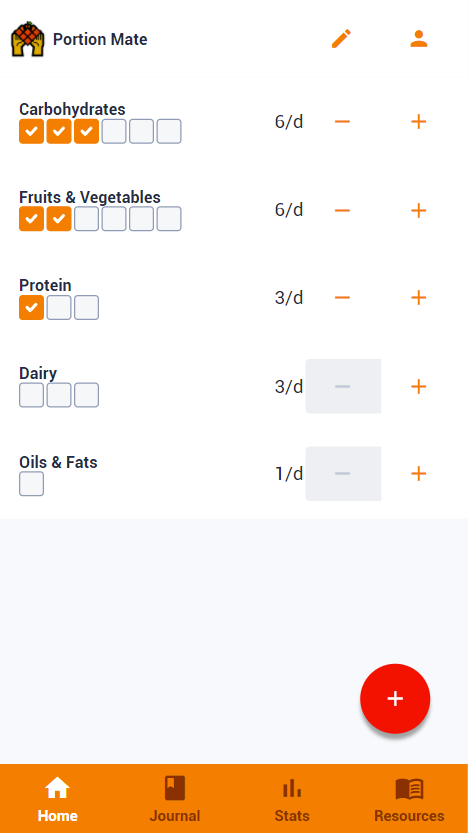
\includegraphics[height=7cm]{interface/Landing [light].png}}
    \caption{Home Page}
    \end{subfigure}\hfill
    \begin{subfigure}{.3\textwidth}
    \centering
    \frame{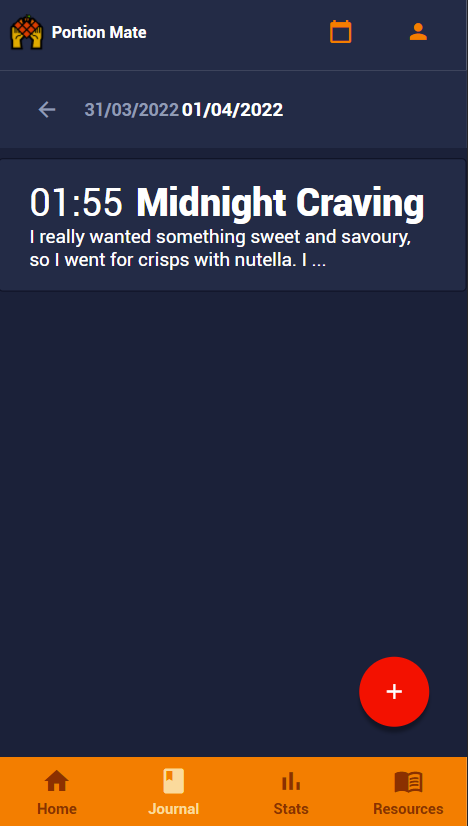
\includegraphics[height=7cm]{interface/Journal [dark].png}}
    \caption{Journal}
    \end{subfigure}\hfill
    \begin{subfigure}{.3\textwidth}
    \centering
    \frame{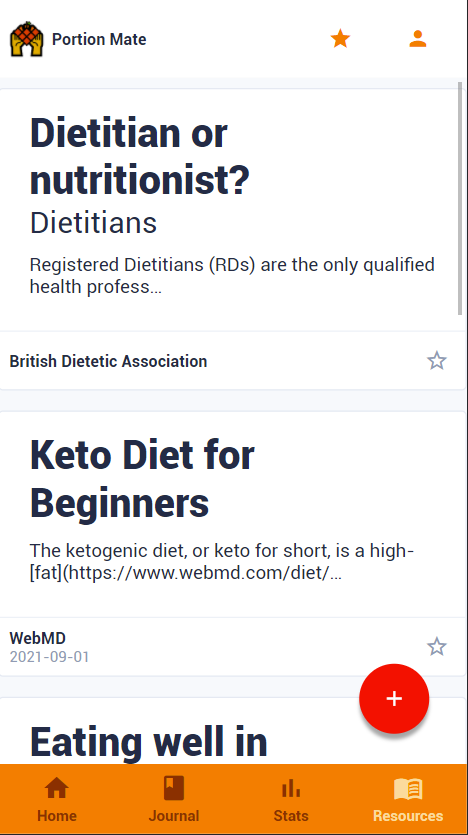
\includegraphics[height=7cm]{interface/Resources [light].png}}
    \caption{Resources}
    \end{subfigure}
    \caption{Final implemented interface}%\label{fig:ui_kitten_interface}
\end{figure}

\subsection{Automation}

It is highly desirable and preferred to have many processes automated as manual process require a lot of time and accuracy, making it error-prone and expensive for development. As discussed in section \ref{sec:Version Control}, pipelines and hooks were taken advantage of.

\subsubsection{Pipelines}

\citetitle{FeaturesGitHubActions} is an incredibly easy and modular approach to setup continuous integration and delivery. Each configuration for an action is called a workflow, and a workflow can have multiple jobs; these must be defined in YAML (example \ref{lst:B.2}). The project defined 12 workflows (figure \ref{fig:5.5}) at the time of writing, each for different purpose which would include testing code functioning \& styling, and the repository issue management (as mentioned in \ref{subsec:Issue Branching}).

\begin{figure}
    \centering
    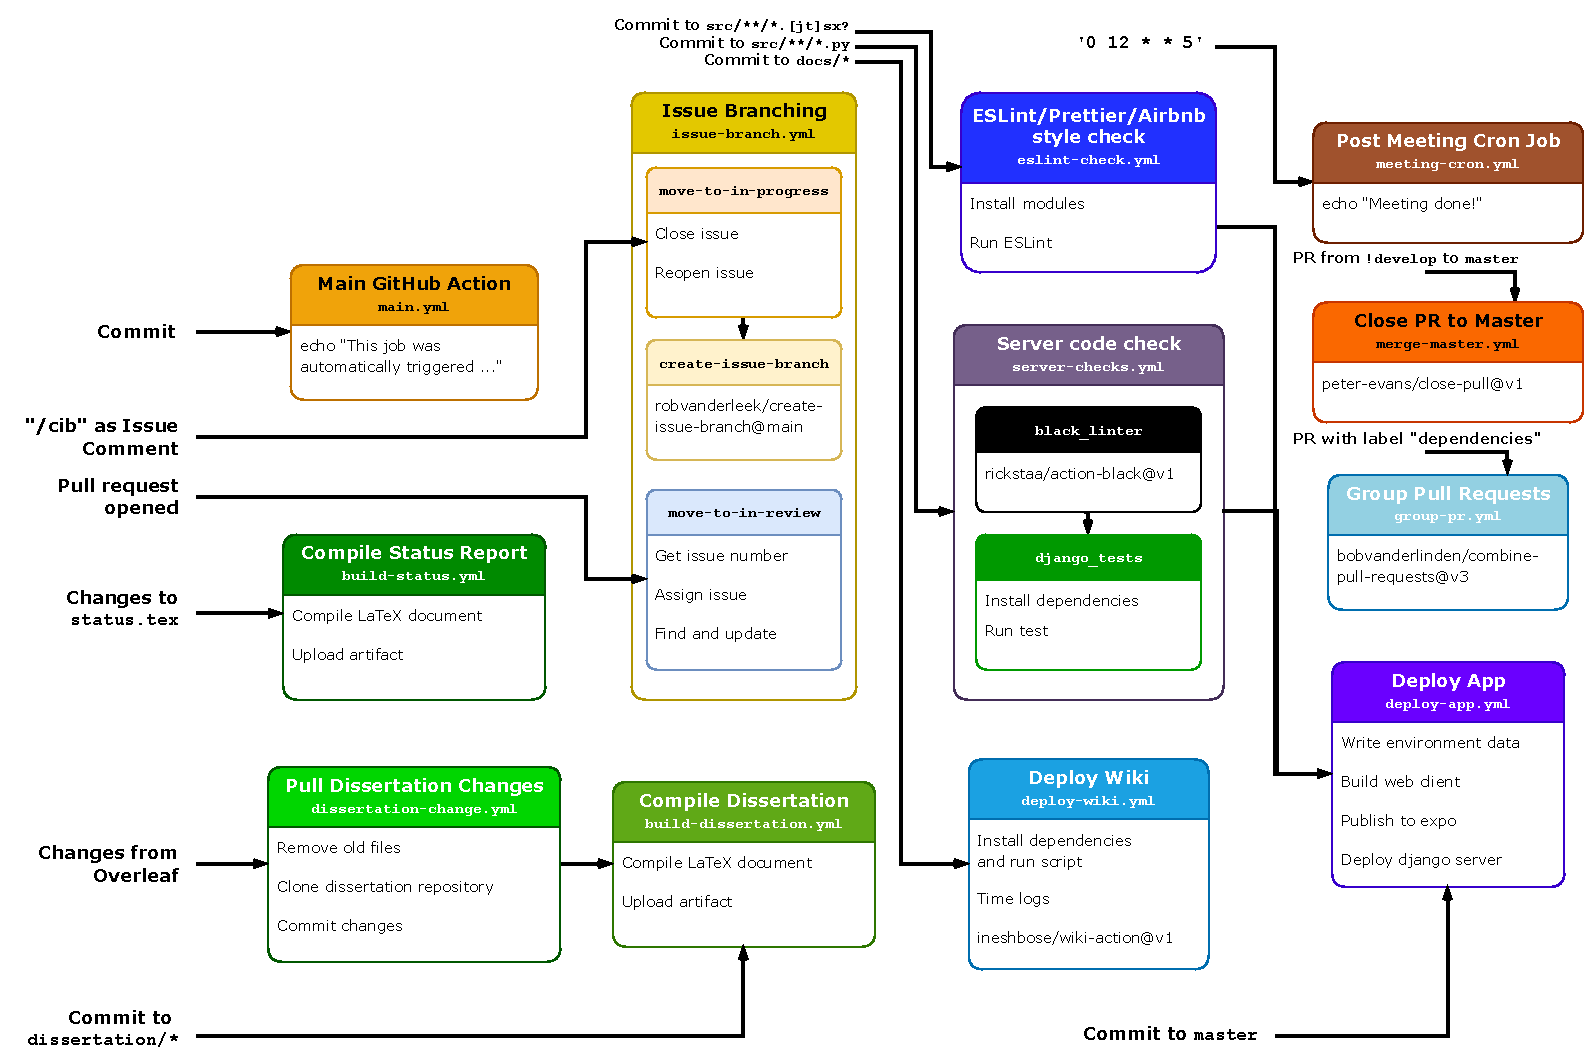
\includegraphics[width=\textwidth]{diagrams/github_workflows.pdf}
    \caption{High level flowchart for the configured pipelines}%\label{fig:workflows}
\end{figure}

\subsubsection{Services}

Additionally, the project also made use of services that aid software development by providing unique features like static analysis, free hosting, or online compilers.

\begin{itemize}
    \item \textbf{\citetitle{codeclimate}} judged the maintainability of the whole codebase and give a suitable grade and estimate it would take to fix issues. At the time of writing, the report gives the repository A grade for maintainability with 0 minutes required to fix issues after breaking down 250 files, finding 0 code smells, duplication and other issues.
    \item \textbf{\citetitle{DevOpsIntelligencePlatform}} also looks for issues in the repository and grades the code quality. At the time of writing, the grade given is an A with four issues indicating three class methods that the analyser feels could be defined as independent functions instead and a super-method being invoked in an unpreferred way.
    \item \textbf{\citetitle{WelcomeReadDocs2022}} allowed the documentation for the application to be build and hosted on the platform, making use of Mkdocs that converts the Markdown files into HTML.
    \item \textbf{\citetitle{Overleaf}} enabled development for reports and documents\footnote{Including this dissertation.} in \TeX through the online editor environment that manages packages and compiles the source.
\end{itemize}

Other services include \citetitle{SnykDeveloperSecurity2020}, \citetitle{LibrariesOpenSource}, and \citetitle{Dependabot2022} for secure dependency management, along with potential usage of \citetitle{AppVeyor} and \citetitle{HomepageTravisCI} for further testing.

\section{Challenges}

With such an intense development in place, a lot of challenges were faced. All were listed as issues on the repository, so those that are not yet closed may not have been solved, and some also had solutions that were not as good as desired.

\subsection*{Setup}

First, while setting up the repository, the workflows had to be configured and there was not a lot of experience with YAML, and it was the first time using GitHub Actions. Since this feature was also released a few years ago, there are still plenty of solutions in development aside from the 12,557 actions already listed on the GitHub Marketplace. This includes the full integration of issue branching (from creating a named branch to closing a linked pull-request, all while automating the linked card on the Kanban board). Fortunately, a lot of research, study and determination enabled the setup in time for main development.

\subsection*{Workspaces}

At the beginning, the repository had separate directories for the Django server (\code{src/backend}) and the React app (\code{src/frontend}). Working on them always required having to change directory, and managing different directories was becoming complex (see \citecode{Issue71}). It was important to have workspaces as the approach for directory organisation was a monorepo (discussed in \ref{subsubsec:Yarn}). The dependency management Poetry (for Python) had limitations of the features than Yarn (for Node.js) offered, like workspaces. This was turned around by reading documentations and having discussions on their support channel, eventually defining sub-packages "\code{portion-mate-src}" \& "\code{portion-mate-docs}", and updating the lock file through hooks, therefore restructuring the repository midway through the project (see \citetitle{pull79}). Overleaf's editor also had limitations like not supporting symbolic link ("\textit{symlinks}") or resolving conflicts, and therefore the \code{dissertation} workspace had to be exported to a separate repository, but continue reflecting changes on the monorepo (see \citecode{issue70}).

\begin{figure}
    \centering
    \noindent\begin{subfigure}{.49\textwidth}
    \begin{lstlisting}[language=toml, caption={Including the sub-packages as dependencies in \citecode{pyprojecttoml}}]
    [tool.poetry]
    name = "portion-mate"
    version = "1.0.0"
    description = ""
    authors = []
    
    [tool.poetry.dependencies]
    python = "^3.8"
    portion-mate-src = {path = "./src"}
    portion-mate-docs = {path = "./docs"}
    \end{lstlisting}
    \end{subfigure}\hfill
    \begin{subfigure}{.49\textwidth}
    \begin{lstlisting}[language=json, caption={Including the directories as workspaces in \citecode{PackageJson}}]
    {
      "name": "portion-mate",
      "version": "1.0.0",
      "main": "src/index.js",
      "private": true,
      "workspaces": [
        "src",
        "docs"
      ], ...
    }
    \end{lstlisting}
    \end{subfigure}
    \caption{examples of Card components}
\end{figure}

\subsection*{Bootstrapping}

For the React Native app, there were greater difficulties. Despite following the traditional TypeScript React approach, there came another learning curve for React Native as it does not offer all features of React, but also requires testing on more devices. Expo (see \ref{subsubsec:Expo}) has been very helpful, however, a critical functionality was the ability to use CSS in React to style elements.

Most code written deals with components and interface layout. Styling libraries provide methods to make design and development easier, for example \citetitle{ottoBootstrap} is one of the most popular frontend frameworks that provides CSS classes like \code{navbar}, \code{float-start} and \code{bg-primary} that would set and style elements accordingly (as the class names would suggest).

\begin{lstlisting}[language=html, caption={Example of a Card element as \href{https://getbootstrap.com/docs/5.1/components/card/\#example}{documented on Bootstrap v5} \cite{Cards}}]
<div class="card" style="width: 18rem;">
  <img src="..." class="card-img-top">
  <div class="card-body">
    <h5 class="card-title">Card title</h5>
    <p class="card-text">Some quick example text to build on the card title and make up the bulk of the card's content.</p>
    <a href="#" class="btn btn-primary">Go somewhere</a>
  </div>
</div>
\end{lstlisting}

For component-based frameworks like React and Vue, such libraries also get extended to provide additional functionality. In this example, \citetitle{ottoBootstrap} would have \citetitle{ReactBootstrap} (for React) and \citetitle{BootstrapVue} (for Vue) where, instead of using classes, components are predefined with lots of additional configuration options using events (\code{onClick}, \code{onHover}) and property parameters.

\begin{figure}
    \centering
    \noindent\begin{subfigure}{.49\textwidth}
    \begin{lstlisting}[language=html, caption={\href{https://react-bootstrap.github.io/components/cards/\#basic-example}{React-Bootstrap} \cite{CardsReactBootstrap}}]
    <Card style={{ width: '18rem' }}>
      <Card.Img variant="top" src="..." />
      <Card.Body>
        <Card.Title>Card Title</Card.Title>
        <Card.Text>
          Some quick example text to build
          on the card title and make up the
          bulk of the card's content.
        </Card.Text>
        <Button variant="primary">
            Go somewhere
        </Button>
      </Card.Body>
    </Card>
    \end{lstlisting}
    \end{subfigure}\hfill
    \begin{subfigure}{.49\textwidth}
    \begin{lstlisting}[language=html, caption={\href{https://bootstrap-vue.org/docs/components/card\#overview}{BootstrapVue} \cite{CardsBootstrapVue}}]
    <b-card
      title="Card Title"
      img-src="..."
      img-top
    >
      <b-card-text>
        Some quick example text to build on
        the card title and make up the bulk
        of the card's content.
      </b-card-text>
      <b-button href="#" variant="primary">
        Go somewhere
      </b-button>
    </b-card>
    \end{lstlisting}
    \end{subfigure}
    \caption{Examples of Card components}
\end{figure}

Unfortunately, this does not translate for React Native, since most of the utilities have been made possible through CSS classes and mobile development does not use HTML or CSS \cite{StyleReactNative}. There are limited components available for native development, like View, Text and Image, and these can only be styled using certain allowed properties, like margins, border and flex (similar to CSS but not the same). This would pose lots of difficulties in the interface development. The library mentioned in section \ref{subsubsec:UI Kitten} helped and aided development, and it was adopted in the middle of development (see \citecode{Issue93}). However, at certain points, extra custom styling had to be added and that also seemed to be repetitive, whereas Bootstrap has a simple class mechanism. Inline styling is not good practice, and for React Native also causes performance issues \cite{StyleReactNative}. Therefore, a React Native equivalent for Bootstrap was developed so that components can use the defined "classes" (see \ref{fig:5.8}, \citecode{Issue116} and \citecode{PullRequest120}).

\begin{lstlisting}[language=typescript, caption={Custom style function in \citecode{SrcAppConstants}}]
const PROVIDED_STYLES = <GlobalStyleSheet>{
  ...spacingStyles,
  ...displayStyles,
  ...flexStyles,
};

export default function createStyle<
  T extends StyleSheet.NamedStyles<T> | StyleSheet.NamedStyles<any>
>(styles: T | StyleSheet.NamedStyles<T>) {
  return StyleSheet.create({ ...PROVIDED_STYLES, ...styles });
}
\end{lstlisting}

\begin{figure}
    \centering
    \noindent\begin{subfigure}{.49\textwidth}
    \begin{lstlisting}[language=html, caption={using inline styles}]
    <div style="display: flex;">
      <div
        style="
          display: flex;
          align-items: 'center';
          justify-content: 'center';
          padding: 2;
        "
      >
        <!-- Spinner CSS is complex -->
        <div style="..."></div>

        <h3>Loading</h3>
      </div>
    </div>
    \end{lstlisting}
    \end{subfigure}\hfill
    \begin{subfigure}{.49\textwidth}

    \begin{lstlisting}[language=html, caption={using Bootstrap classes}]
    <div class="d-flex">
      <div
        class="
          d-flex
          align-items-center
          justify-content-center
          p-2
        "
      >
        <div class="spinner-border"></div>
        <p class="fs-3">
          Loading...
        </p>
      </div>
    </div>
    \end{lstlisting}
    \end{subfigure}
    \vskip\baselineskip
    \noindent\begin{subfigure}{.49\textwidth}
    \begin{lstlisting}[language=html, caption={usage with inline styles (through objects) causing increased complexity (bad practice) \cite{StyleReactNative}}]
    <SafeAreaView style={{ flex: 1 }}>
      <Layout
        style={{
          flex: 1,
          alignItems: 'center',
          justifyContent: 'center',
          padding: 2,
        }}
      >
        <Spinner size="giant" />
        <Text style={styles.title}>
          {'Loading...'}
        </Text>
      </Layout>
    </SafeAreaView>
    \end{lstlisting}
    \end{subfigure}\hfill
    \begin{subfigure}{.49\textwidth}

    \begin{lstlisting}[language=html, caption={example of usage like Bootstrap in \citecode{SrcAppNavigation}}]
    <SafeAreaView style={styles.flex1}>
      <Layout
        style={[
          styles.flex1,
          styles.alignItemsCenter,
          styles.justifyContentCenter,
          styles.padding2,
        ]}
      >
        <Spinner size="giant" />
        <Text style={styles.title}>
          {'Loading...'}
        </Text>
      </Layout>
    </SafeAreaView>
    \end{lstlisting}
    \end{subfigure}
    \caption{Effect of Bootstrap, in HTML code (above), and React \textbf{Native} code (below; \code{display:'flex'} is not native)}%\label{fig:bootstrap_effect}
\end{figure}

\section*{Summary}

The project promised and delivered on a system that would be highly maintainable, modular and robust using the best practices throughout the process, even if that meant implementing solutions from scratch, such as automating issue branches in GitHub through pipelines or dynamically generate style properties for components. This went above and beyond the application, which itself was developed using React Native in TypeScript, accompanied with Expo to distribute on different platforms, and the backend database server using Django, along with PostgreSQL, extended by Django REST Framework to provide API to the frontend clients.

\end{document}
